% !TeX spellcheck = en_GB
\documentclass{egpubl}
\usepackage{wait2020}
%\usepackage{float}

\ConferencePaper      % uncomment for (final) Conference Paper

\title{Controlled human face synthesis with\\
	 \space Generative Adversarial Network}

\author[Hornyák,Póka,Szemenyei]
       {Szabolcs Hornyák$^1$,
        Károly Bence Póka$^2$ and
        Márton Szemenyei$^3$
        \\
        $^1$ Msc student of the Department of Measurement and Information Systems,
             Budapest, Hungary\\
        $^2$ Msc student of the Department of Control Engineering and Information Technology,
        Budapest, Hungary\\
        $^3$ PhD student of the Department of Control Engineering and Information Technology,
       }
%for including postscript figures
\usepackage[pdftex]{graphicx}
% \usepackage[dvips,draft]{graphicx}% replace PS figure by framed file name

\PrintedOrElectronic

% prepare for electronic version of your document
\usepackage{t1enc,dfadobe}

% For backwards compatibility to old LaTeX type font selection.
% Uncomment if your document adheres to LaTeX2e recommendations.
\let\rm=\rmfamily    \let\sf=\sffamily    \let\tt=\ttfamily
\let\it=\itshape     \let\sl=\slshape     \let\sc=\scshape
\let\bf=\bfseries

% if the Editors-in-Chief have given you the data, you may uncomment
% the following five lines and insert it here
%
% \volume{22}   % the volume in which the issue will be published;
% \issue{3}     % the issue number of the publication
% \pStartPage{???}      % set starting page
\usepackage{amsmath}
\usepackage{amsfonts}
\begin{document}

\maketitle

\begin{abstract}
Classical data augmentation techniques are not sufficient for facial recognition problems with small datasets. In this paper we present our work aimed to develop generative models for data augmentation. We studied several GANs that provide control over the features of the generated images, then tried to implement a model that can be used for altering attributes of real images. We experimented with multiple architectures, studied the effects of certain loss functions and the practical limits of image recovery. Our attempts moved towards the aforementioned goal but was not reached during the semester. At last we found but did not come to thoroughly examine great methods to improve the quality of the generated images. We will continue to develop our solution with these methods and the experience gained from the project.

%\begin{classification} % according to http://www.acm.org/class/1998/
%\CCScat{I.3.3}{Computer Graphics}{Line and Curve Generation}
%\end{classification}

\end{abstract}

\section{Introduction}

Facial recognition is a popular field  of deep learning nowadays. Numerous methods and network architectures have been developed and applications range from authentication and security to diagnosing certain medical conditions.

One of the main problem of deep learning applications is data shortage, and it is also frequent in facial recognition. For example to train a neural network to recognize the rightful owner of the car it is embedded into would require an impossible amount of image data from the driver. The problem can be addressed by use of transfer learning methods and/or data augmentation techniques. While transfer learning is a great way to exploit the capabilities of pretrained models, changes in facial attributes such as growing a beard or getting glasses would require the system to adapt by retraining itself. Use of data augmentation faces the same problem because its image transformations do not alter the features of the given image.

Our solution is aimed towards generative data augmentation to address the above mentioned problems. We examined and extended improved versions of the InfoGAN architecture to generate and regenerate high quality images and controlling their features in the latent space. This approach enables the original dataset to be augmented in a meaningful way, generating images of the same face with different features. Because components of the latent vector can be connected to facial attributes, data augmentation becomes the exploration of the latent space in different directions.

After the theoretical basis of generative networks we list the existing GAN architectures that provide control over image attributes. Then we describe our extensions and modifications made to these architectures and present the results.


\section{CelebA dataset}

For the training of every model we used the Large-scale CelebFaces Attributes (CelebA) dataset. This set contains 202599 celebrity images, each with 40 attribute annotation but we only used the pure cropped images without annotation. CelebA has a large diversity and quantity. We can find faces with glasses, in various poses and with different mimics. The cropped size of the images is 178x218 which seems poor but the dilemma of the generation size can be easily a memory consuming problem.


\section{Basic theory of GANs}
The abbreviation "GAN" stands for Generative Adversarial Network and it was published by Goodfellow et al. \cite{goodfellow2014generative} in 2014. It comprises of a generator and a discriminator network. These networks compete during training:

\begin{itemize}
	\item the objective of the discriminator is to distinguish between real and generated images,
	\item the objective of the generator is to fool the discriminator by generating images indistinguishable from real ones. 
\end{itemize}

These opposing objectives can be formulated as:

\begin{equation}
\begin{aligned}
\min_G \max_D V(D,G) &= \mathbb{E}_{x\sim p_{data}(x)}\left[ \mathrm{log}D(x) \right] \\
&+ \mathbb{E}_{z\sim p_{z}(z)}\left[ \mathrm{log}(1-D(G(z)))\right]
\end{aligned}
\end{equation}

During training we alternate between $k$ steps of optimizing the discriminator and one step of optimizing the generator network, where $k$ is a hyperparameter usually set to 1.

The GAN architecture provided much better results then previous methods. The downside of the "vanilla" GAN architecture is that the representation of image features in the latent space become highly entangled \cite{radford2015unsupervised}, hence any change made to the latent vector will effect multiple attributes of the generated image. Because the basic architecture of GANs does not provide control over the features of the generated images we looked for more advanced architectures.


\subsection{InfoGAN}

The first network we examined was the InfoGAN by Chen et al. \cite{chen2016infogan} and some of its improved versions \cite{10.1007/978-3-319-78452-6_5}\cite{mirza2014conditional}. This generative architecture attempts to control the features of the generated images via so called code components concatenated to the latent (noise) vector. In order to encourage the generator to connect these code components to meaningful image features (to learn a disentangled representation) the authors introduced a new criteria in the generator's loss function: the generator should maximize the mutual information between the input latent vector and the generated image.

The total loss of the generator ($L_G$) is defined as:

\begin{equation}\label{g_loss}
L_G = -L_D(x_G) - \lambda I([z,c], x_G)
\end{equation}
where $L_D(x_G)$ is the loss of the discriminator for generated images, $I([z,c], x_G)$ is the mutual information between the latent vector and the generated image, $\lambda$ is a new hyperparameter, typically 1.

The InfoGAN architecture provides great control over the image features if the type and number of code components are suited to the underlying distribution of the dataset (e.g. use of a categorical component with 10 categories for MNIST). The downside of this architecture is the relative poor quality of the generated images for complex data such as faces from the CelebA dataset. The architectures described below attempts to address this problem and to further remove the entanglement of features in the latent space.


\subsection{ST-GAN}
\label{sec:propDet}

One improvement of the InfoGAN architecture is called Semantic Transformation GAN \cite{liu2019stgan}. This networks aims to remove the complicated procedure of approximating the mutual information by introducing an encoder network. The task of this encoder network is to reconstruct the latent vector presented to the generator from the image it generated. This can only be achieved if the generator preserves the latent vector's information in the generated images. In other words, perfect $[z,c]$ reconstruction can only be achieved if the information flow from the input of the generator to the output of the encoder is lossless, and it also means that the generator maps all the information of the latent vector into the generated images.

One can use the ST-GANs encoder network to map an existing image into the latent space, then alter its code components and feed the altered vector to the generator in order to generate an altered version of the original image. With the above described architecture the quality of the altered images are not guaranteed. To overcome this problem the authors of the paper used the reconstructed $[z,c]$ vector from the encoder, altered it ($[z,c']$) and fed back into the generator during training, and defined another objective for the network to improve the quality of the altered images.

This architecture is a significant improvement of InfoGAN, but it has a relatively large number of subnetworks to train and loss functions. Latter leads to conflicting training objectives and slower convergence.

\begin{figure*}[!htb]
	\centering
	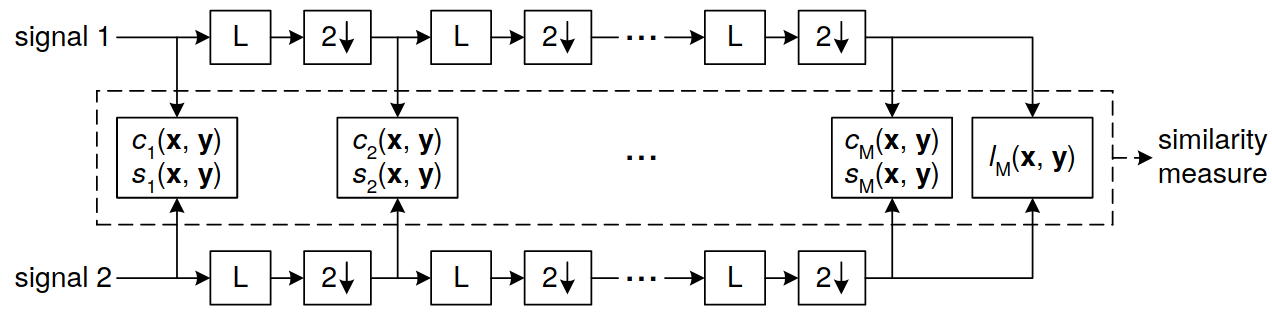
\includegraphics[width=\textwidth]{pic/MS-SSIM}
	\caption{Multi-scale SSIM system, L: low-pass filter, 2$\downarrow$: downsampling by 2 (image source: \cite{1292216})}
	\label{fig:ms_ssim}
\end{figure*}


\subsection{BEGAN}
\label{sec:digErr}

A further improved InfoGAN-based architecture is called the Boundary Equilibrium GAN \cite{berthelot2017began}.

Because at the beginning of the training the generator creates images greatly different from the real images the discriminator has an advantage. To overcome this and assure "fair play" between these networks the BEGAN architecture introduces a balancing process, hence the name "boundary equilibrium".

The BEGAN architecture also uses the idea of latent vector reconstruction to remove the need to approximate the true mutual information, but uses a whole autoencoder network as a discriminator.

The discriminator, as an autoencoder has the objective to perform good on real images and bad on generated ones, hence the quality of the reconstruction can be used to discriminate between real and fake images. By this discriminator implementation, the generator is heavily encouraged to produce images with same distribution and same properties as real ones, resulting in better results than previous architectures can achieve.

The only shortcoming of this architecture is that it cannot be used to alter features of real images. Its autoencoder network cannot be used to reconstruct the $[z,c]$ latent vector presented to the generator because it learns a totally different representation of the data. This was one of our main problem using the BEGAN architecture and we had to extend it in order to both reach our goal and exploit the BEGANs capabilities to generate high quality images.


\section{The whole development process}
%\label{appendix:development}

\subsection{InfoGAN-based models}

At first, to get familiar with the problem we tried to solve we started the development process with examining the original InfoGAN paper and existing implementations. Our first network was a simple InfoGAN implementation based on these sources \cite{chen2016infogan}. To start from a simple problem we generated MNIST-like images. The results were promising, because we successfully reproduced the results presented in the InfoGAN paper for MNIST.

\begin{figure}[!htb]
	\centering
	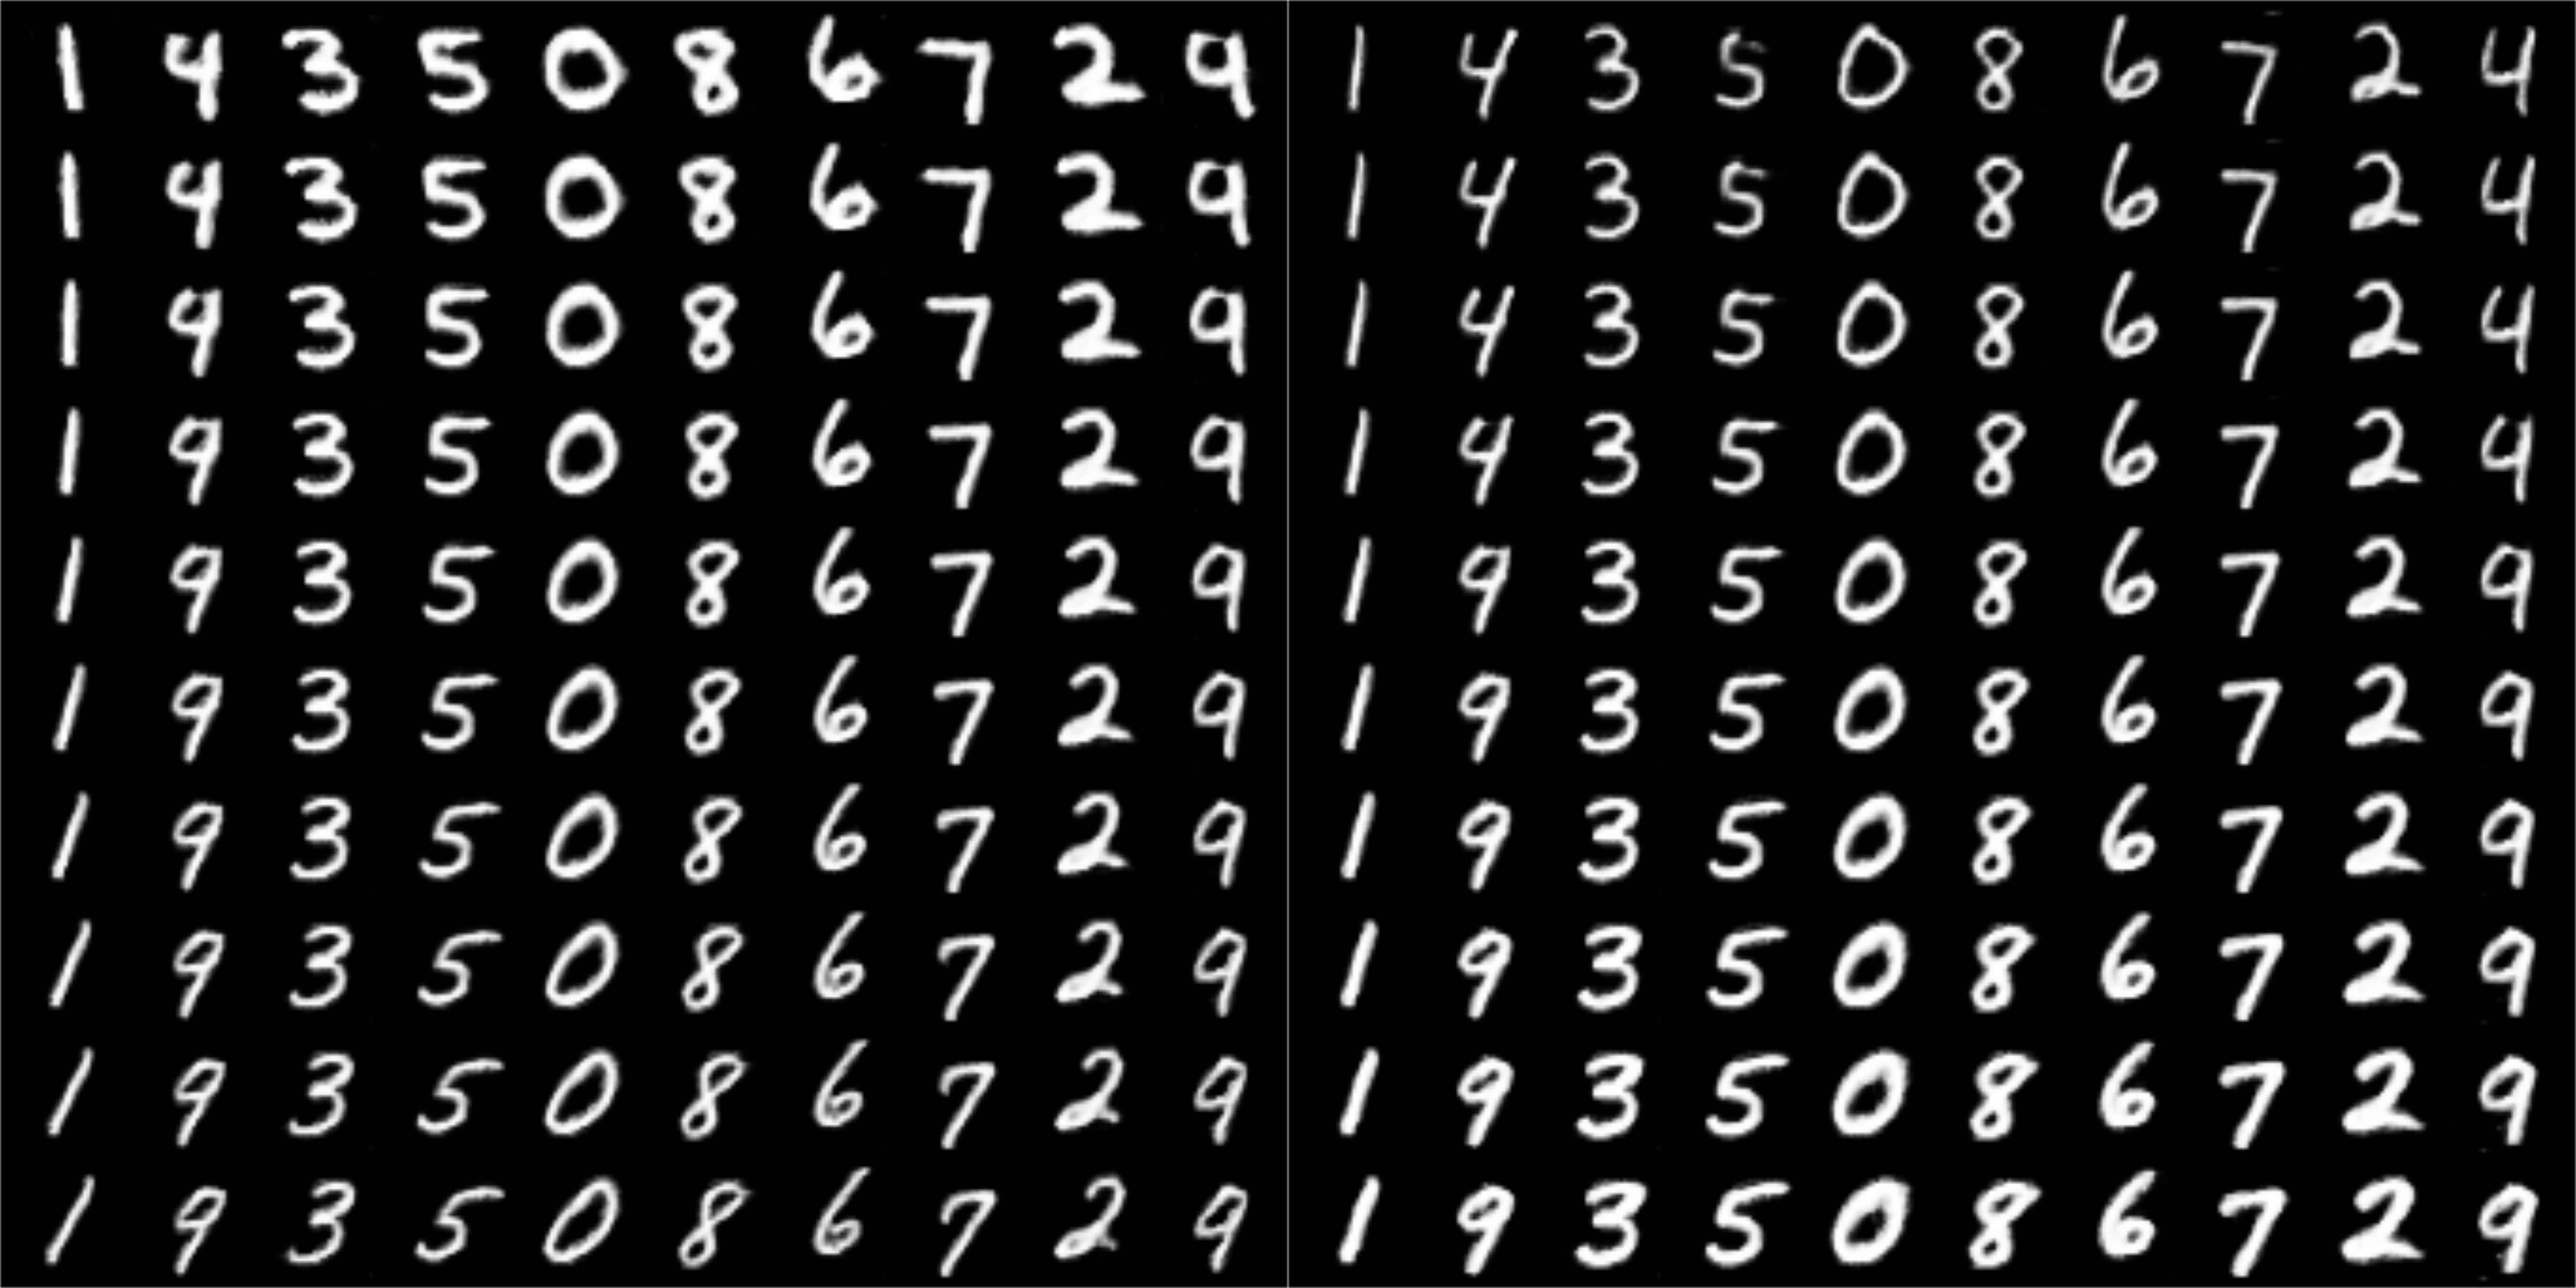
\includegraphics[width=1\linewidth]{pic/mnist}
	\caption{First feature-controlled generation for handwritten digits. Each column corresponds to one state of the categorical code component, controlling which digit is being generated. On the left, $c_1$ continuous component varies controlling the angle of the written digits, while at the right, $c_2$ varies controlling the thickness of the digits.}
	\label{fig:mnist_results}
\end{figure}

The next step was to switch dataset and to try to generate controlled images of celebrities. We started with a picture size of 64x64 pixel and managed to generate mid-quality images.

\begin{figure}[!htb]
	\centering
	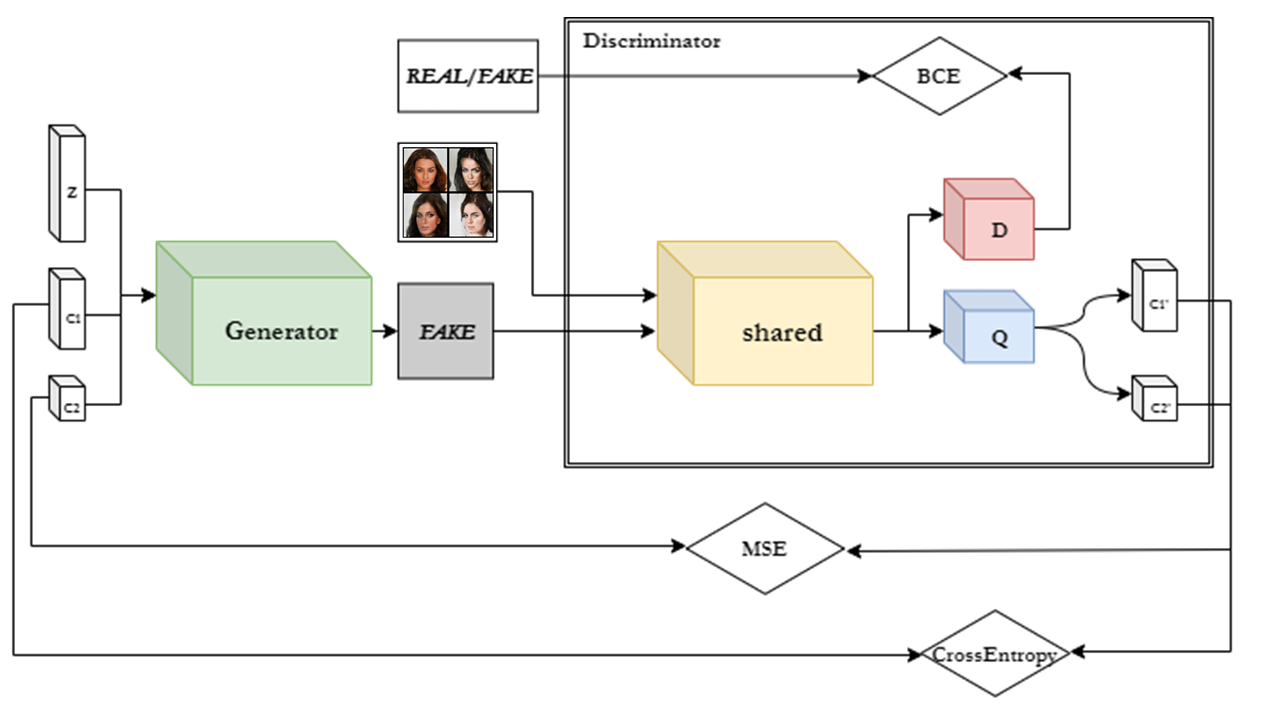
\includegraphics[width=\linewidth]{pic/1}
	\caption{First InfoGAN implementation}
	\label{fig:infogan}
\end{figure}

\subsection{Our extensions and improvements}
The main goal was impossible to achieve with the existing architectures, because we wanted to fine-tune a given picture, but the generator has a multidimensional vector input. Our idea was to train a separated predictor to get noise and code vectors from a given pictures.  At first two questions come up: what the predictor net’s output should be? Could be whether we can use the Discriminator as a predictor, because it can give us a categorical and continuous code from a given image. The answer is not. The Discriminator was trained to give a judgment about the classification (True or Fake), and the appropriate code vectors. We can not train the Discriminator to give the noise vector also, because that trick would change the training results in a bad way. So, let’s make a Noise Predictor net.

We used a network based on a same architecture as the Generator has but with noise, categorical and continuous code as outputs. Our network object has on opportunity to train only the predictor network. We trained the InfoGan first and then fine-tuned the Noise Predictor with the Generator weights. At first, we used the built-in pytorch MSE (Mean Square Error) loss function to compute the loss between the generated image based on the predictor’s output and the original image. The mathematically distance between the pixels does not always show the visible difference for humans between two pictures. Therefore, we used the Differentiable Multi-Scale Structural Similarity (SSIM) index to calculate the predictor’s loss.



\begin{displaymath}
\mathrm{MS\mbox{-}SSIM}(x,y) = I_M(x,y)^{\alpha_M} \prod_{j=1}^{M} C_j(x,y)^{\beta_j}S_j(X,y)^{\gamma_j}
\end{displaymath}

Obviously, the goal is for the network to learn to produce visually pleasing images. To the root of the MS-SSIM is the simple SSIM function. Where for pixel p is defined as 

\begin{equation}
\begin{aligned}
\mathrm{SSIM}(p) &= \frac{2\mu_x\mu_y + C_1}{\mu_x^2 + \mu_y^2 + C_1}\cdot\frac{2\sigma_{xy} + C_2}{\sigma_x^2 + \sigma_y^2 + C_2} \\ 
&= l(p)\cdot cs(p)
\end{aligned}
\end{equation}

Means ($\mu$) and standard deviations ($\sigma$) are computed with a Gaussian filter with standard deviation $\sigma_G$. The max output of this metrics is 1 when the two inputs are similar to each other and the minimum is 0 when they are not. In the training loop we can use the loss function like this:

\begin{equation}
\mathcal{L}^{\mathrm{SSIM}}(P) = \frac{1}{N}\sum_{p \in P}1-\mathrm{SSIM}(p)
\end{equation}

where the p is the pixel and we are looking at its neighbourhood as large as the support of the G ($\sigma_G$). So, we can write the loss as

\begin{equation}
\mathcal{L}^{\mathrm{SSIM}}(P) = 1-\mathrm{SSIM}(\tilde{p})
\end{equation}

because the convolutional nature of the network, where the $\tilde{p}$ is the centre pixel of patch P. 
The processed quality depends on the size of $\sigma_G$, but rather then fine-tuning it we can use MS-SSIM. Further information you can visit the cited source of Nvidia Resource \cite{zhao2015loss}.

\begin{equation}
\mathrm{MS\mbox{-}SSIM}(p) = l_M^\alpha \cdot \prod_{j=1}^{M}cs_j^{\beta_j}(p)
\end{equation}



\subsubsection{Extending InfoGAN with noise-vector recovery}

The InfoGAN implementation we based our work on implements the code recovery and discriminator with the use of a shared network: it comprises of the convolutional layers that process the real and fake images, and the code recovery as well as the decision making (discriminator functionality) comes after this common part.

\begin{figure}[!htb]
	\centering
	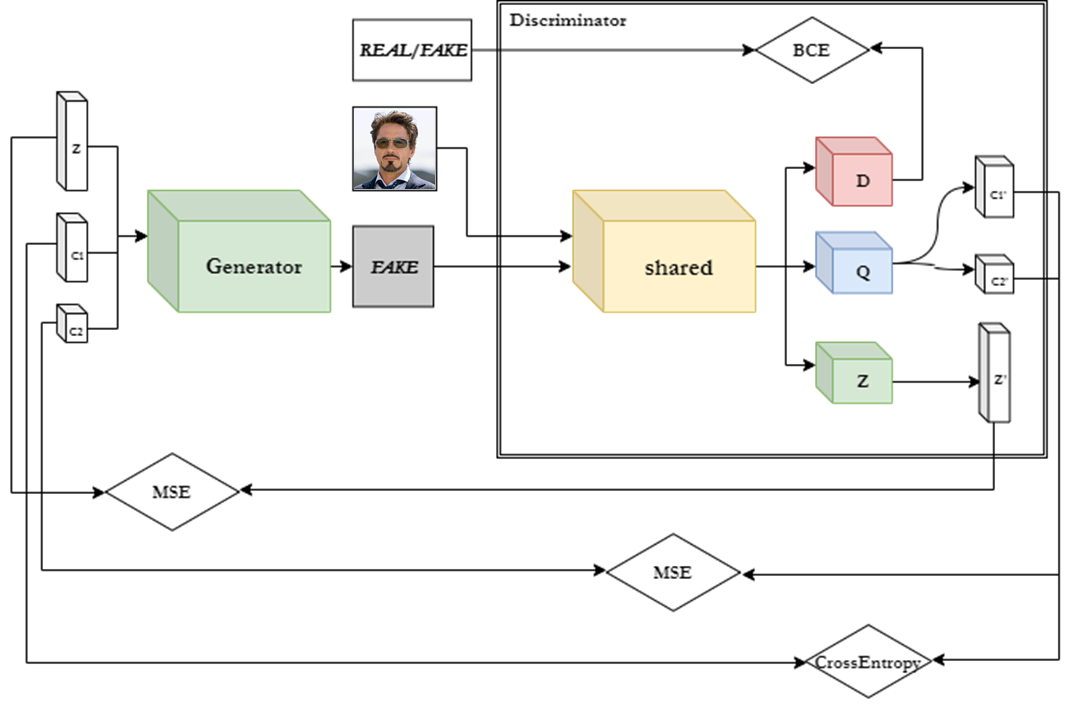
\includegraphics[width=\linewidth]{pic/Infogan_diss_predicting}
	\caption{Extended InfoGAN implementation}
	\label{fig:infogan_simple_noise}
\end{figure}



Because our goal was to alter existing images with our network, the first extension we added to the original InfoGAN was a noise-recovering FC-layer after the shared network, similar to the one used for code recovery. We defined the same L2-loss for this noise predictor just like we did for code recovery, and simply added it to the total info-loss with a 0.1 coefficient.



\begin{figure}[!htb]
	\centering
	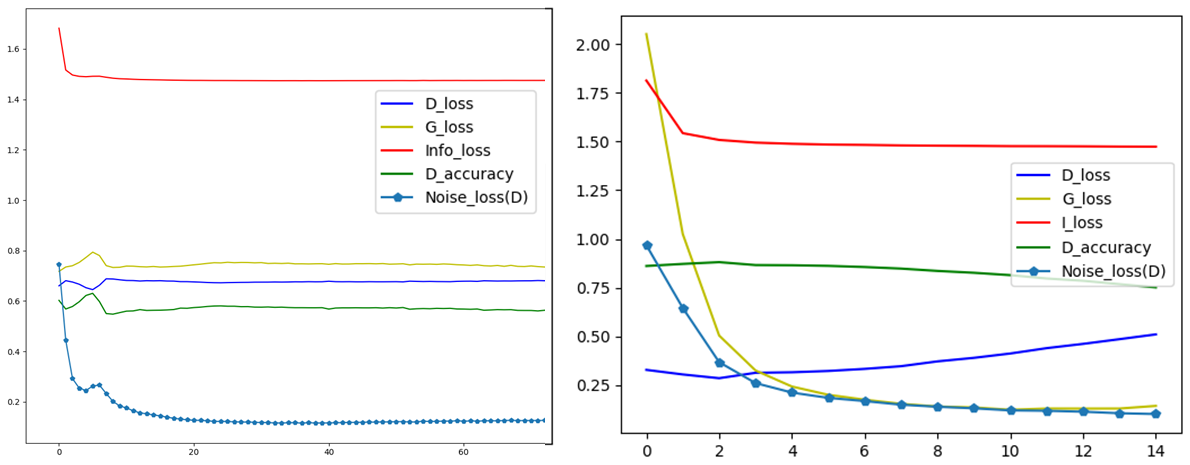
\includegraphics[width=\linewidth]{pic/added_noise2}
	\caption{Improved convergence with disruptive noise on the discriminator's input}
	\label{fig:added_noise}
\end{figure}

\begin{figure}[!htb]
	\centering
	\includegraphics[width=\linewidth]{pic/tony_regen}
	\caption{First image reconstruction results}
	\label{fig:tony_regen}
\end{figure}


\subsubsection{Suppressing the discriminator with added noise}

After multiple training sessions with the extended InfoGAN we realized that at the beginning of the training the discriminator gains too much advantage. The loss of the generator starts from a high value and decreases slowly because it cannot compete with the discriminator.

To disrupt the discriminator we added Gaussian noise to its input. By controlling the power of the added noise we can suppress the discriminator to make room for improvement of the generator.







We started our first hyperparameter optimization session at this point. The hyperparameters and their sets of values were the following:


\begin{itemize}
	\item Image size: \{32x32, 64x64\}
	\item Dimension of the latent vector (noise and code concatenated): \{64, 128\}
	\item Dimensions of categorical code: \{8, 10\}
	\item Noise "power": \{1/15, 1/20\}
	\item Learning rate: \{$10^{-4}, 2 \cdot 10^{-4}$\}
	\item Batch size: \{8, 64, 128, 512\}
	\item Epochs: \{15, 20, 42, 50, 100\}
\end{itemize}

As a result of this optimization process we learned that: 1) one learning rate for all subnetworks may not be the best choice, 2) the image size and the size of the latent vector should change together to maintain quality, 3) batch size largely effects the quality of the generated images, 4) the higher value of noise power is needed for balanced training.

Another problem was the recovery of the noise part of the latent vector. Convergence of noise recovery slowed down then stalled in a state that did not provide sufficient image recovery.

\begin{figure}[!htb]
	\centering
	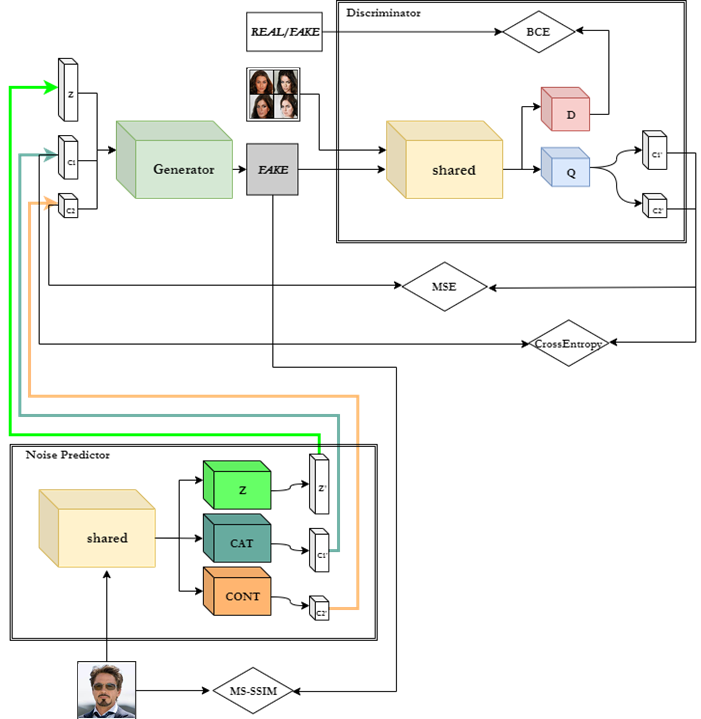
\includegraphics[width=\linewidth]{pic/2}
	\caption{Extended InfoGAN structure with separate predictor network}
	\label{fig:infogan_noise}
\end{figure}



\subsubsection{Separating the discriminator from latent vector recovery network}

After we extended the original InfoGAN architecture and run multiple training sessions we decided to separate the discriminator from the latent vector predictor. We hypothesized that the shared layers cannot be optimized if they had to adapt according to three different objectives and loss functions.



\begin{figure}[!htb]
	\centering
	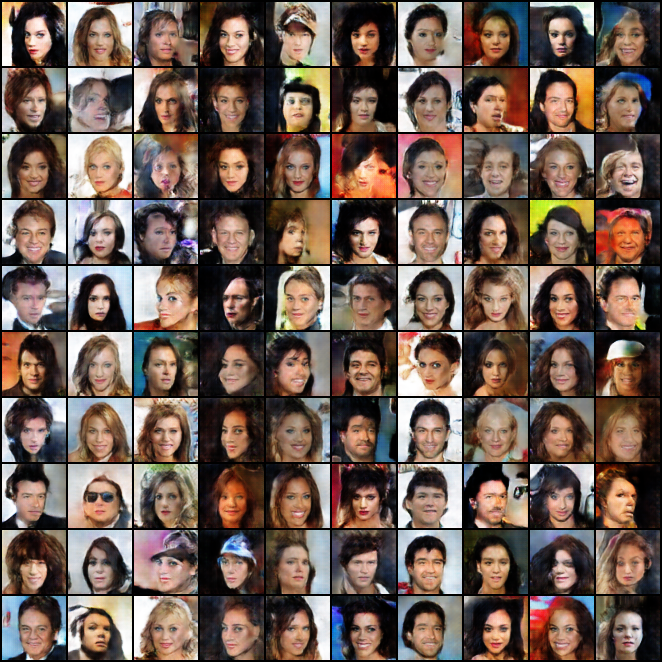
\includegraphics[width=1\linewidth]{pic/best1}
	\caption{Best results from random noise with our InfoGAN-based architecture}
	\label{fig:best1}
\end{figure}

\begin{figure}[!htb]
	\centering
	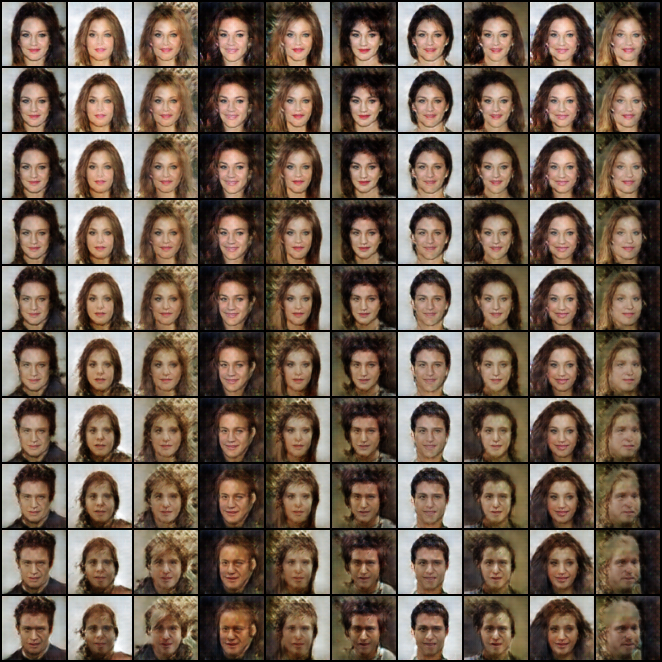
\includegraphics[width=1\linewidth]{pic/best2}
	\caption{Best results of controlled image generation with our InfoGAN-based architecture}
	\label{fig:best2}
\end{figure}



% This is here because this way it will be on the top of the correct page
\begin{figure*}[!ht]
	\centering
	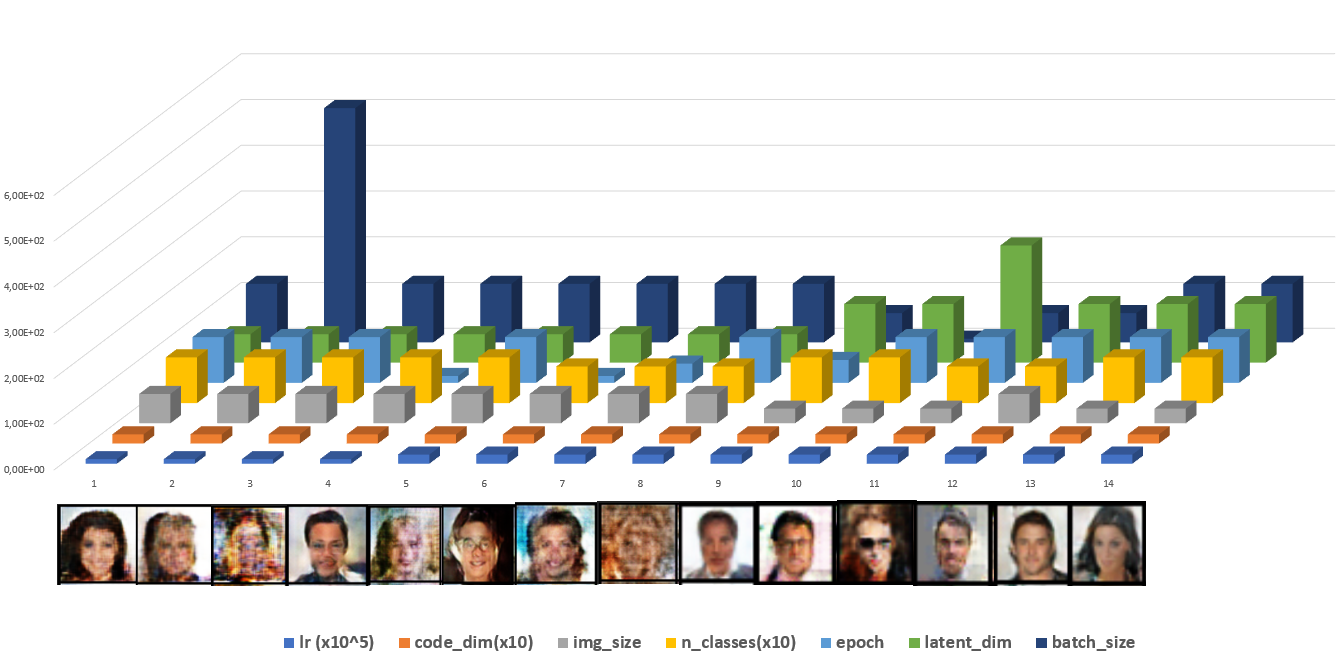
\includegraphics[width=\textwidth]{pic/hyperparamopt}
	\caption{Series of hyperparameter runs}
	\label{fig:hyperparamteres}
\end{figure*}


First, we removed the noise recovery layer and created a new, independent network. This way only two task remained for the discriminator: making a decision about the input image (real or fake) and to recover its control code components (for mutual information maximization).



The next step was to extend the predictor network to predict the whole latent vector of real images that are desired to be altered. The resulting architecture can be seen in Fig. \ref{fig:infogan_noise}. This extended predictor network should become, in theory, the inverse of the generator, effectively forming an autoencoder with it.




Results became better with a slightly faster convergence. To further improve the performance of noise recovery we experimented with some of the hyperparameters, then tried to approximate the practical limit of noise recovery (see below).


\begin{figure}[!htb]
	\centering
	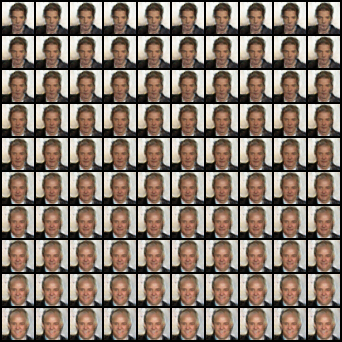
\includegraphics[width=1\linewidth]{pic/predict_everything}
	\caption{Best Tony Stark Reconstructing with our InfoGAN architecture with separated noise predictor (predict everything)}
	\label{fig:best3}
\end{figure}



\subsubsection{Hyperparameter optimization}

During development we experimented with multiple architectures and made several extensions to existing implementations, hence our hyperparameter optimization sessions are distributed and made between architectural changes. As we can see 



\subsubsection{Iterative noise recovery}

To find the limit of the noise recovery to a given generator we tried to iteratively approximate the noise vector. The quality of the recovery highly depends on the resolution of the generated images by the generator.\\


\begin{figure}[!htb]
	\centering
	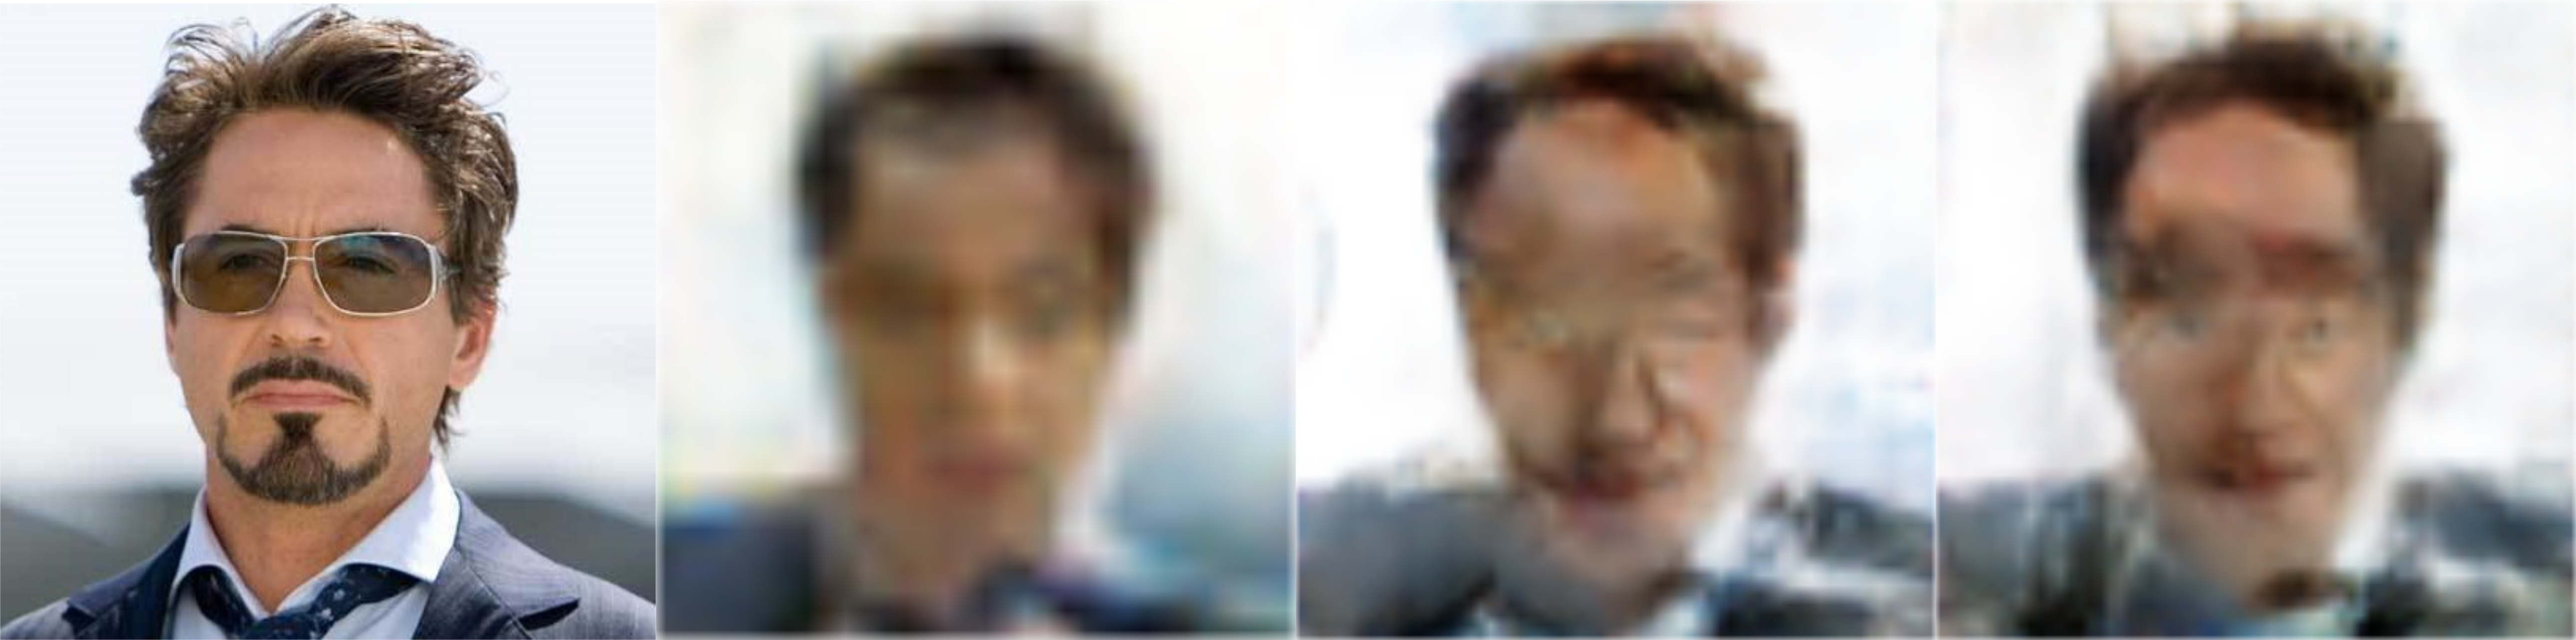
\includegraphics[width=\linewidth]{pic/tony_iterative}
	\caption{Results of iterative noise approximations with different error functions (from left to right): original image, MSE, SSIM, MS-SSIM}
	\label{fig:tony_iterative}
\end{figure}

We tried to fine-tune the latent vector with a generator trained on 32x32 images and 64x64 ones and the latter one proves the theory. We used only the Generator and an Adam optimizer to fine-tune the latent vector. Our goal was to get the appropriate vectors which we can feed to the generator for the desired image generation. We found out that the limit is not yet reached with the noise predictor but the generator is also a limiting factor in the recovery process, hence we started to look for ideas to improve image quality.

\begin{figure}[!htb]
	\centering
	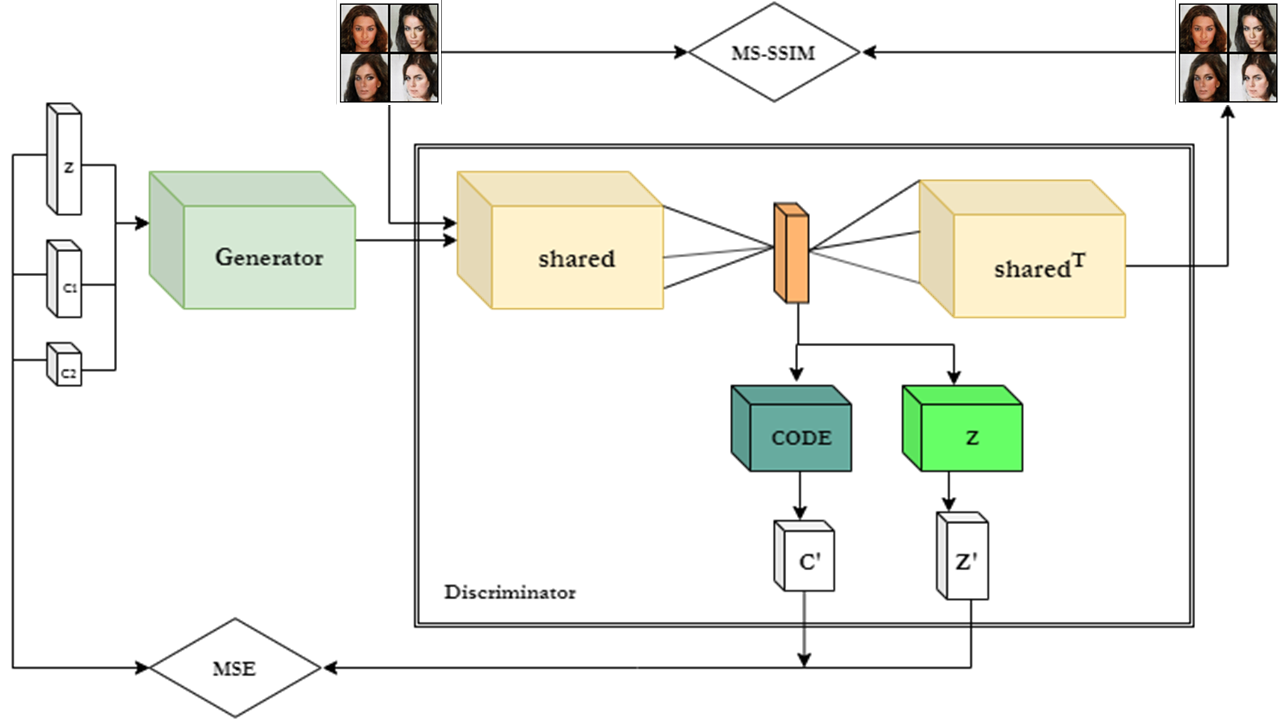
\includegraphics[width=\linewidth]{pic/3}
	\caption{Architecture using autoencoder as discriminator (BEGAN-inspired)}
	\label{fig:infogan_ae}
\end{figure}





\subsubsection{InfoGAN-BEGAN hybrids}

After several attempts to improve image quality of the modified InfoGAN architecture we looked for new architectural ideas. The search ended with the Boundary Equilibrium GAN and the idea of implementing the discriminator as an autoencoder. We examined and merged this idea into our network.

\subsubsection{Using an Autoencoder as discriminator}

Borrowing the idea from the BEGAN architecture we modified our discriminator to form an autoencoder. We used the layers of discriminator for image encoding, and the layers of the generator for decoding. 

Unfortunately, the structure of the previously used subnetworks proved to be suboptimal to form an autoencoder. We tried to make their structure more symmetrical but eventually reached the conclusion that we have to implement the discriminator from scratch.

\subsubsection{Implementing BEGAN and extending it with noise recovery}

After the effectively failed attempt of tailoring the InfoGAN architecture to be more like BEGAN, we tried the other direction: implementing BEGAN and modifying it to meet our goals. We extended an existing implementation with our previously developed predictor network, the resulting architecture can be seen on Fig. \ref{fig:infogan_ae_noise}.

\begin{figure}[!htb]
	\centering
	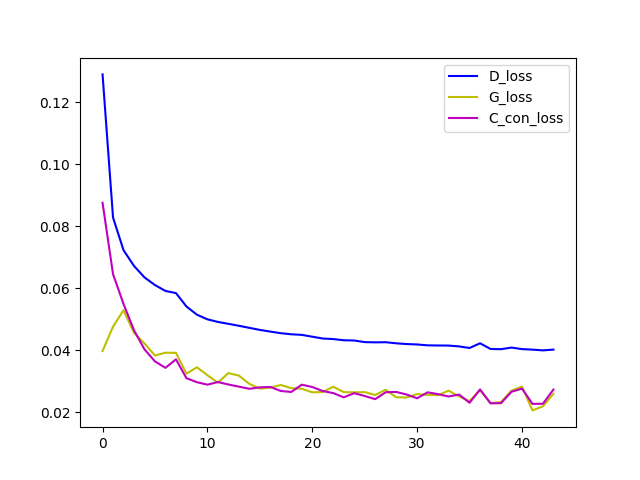
\includegraphics[width=\linewidth]{pic/InfoBegan(proper)}
	\caption{Our implemented structure's losses during training}
	
\end{figure}

\begin{figure}[!htb]
	\centering
	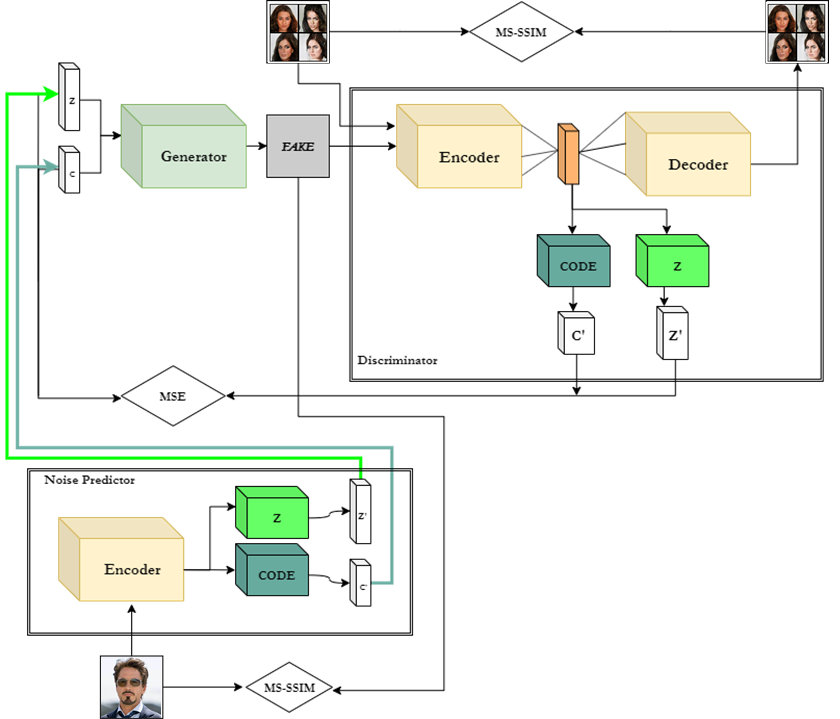
\includegraphics[width=\linewidth]{pic/BInfoGAN+predictor}
	\caption{Architecture using autoencoder as discriminator (BEGAN-inspired) extended with noise predictor network}
	\label{fig:infogan_ae_noise}
\end{figure}

The generated images had better quality than before but we could not control their properties as we originally wanted. We conducted multiple experiments with this network and eventually found out that the base BEGAN implementation may suffers from a minimal mode collapse with the given set of hyperparameters.

\begin{figure}[!htb]
	\centering
	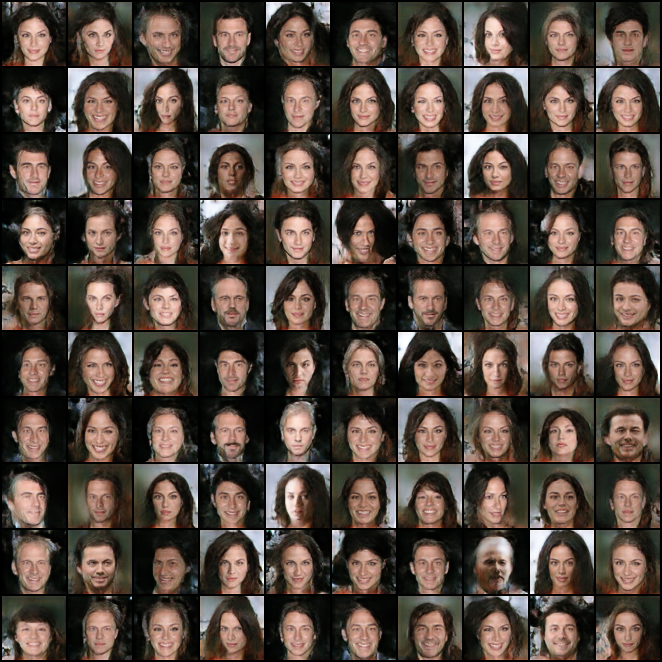
\includegraphics[width=\linewidth]{pic/InfoBegan_random_result}
	\caption{The random generated result of our modified BEGAN structure}
	
\end{figure}

\subsubsection{Improving image quality with advanced loss functions}

To improve the quality of generated images we looked for advanced loss functions to find more meaningful metrics than MSE.

The first candidate was Structural Similarity (SSIM) method. This metric was developed to approximate human perception of image quality and comprises of three components: luminance, contrast and structure. This method is used extensively for iterative latent code approximation and it proved to be better than MSE for our purposes.

\begin{figure}[!htb]
	\centering
	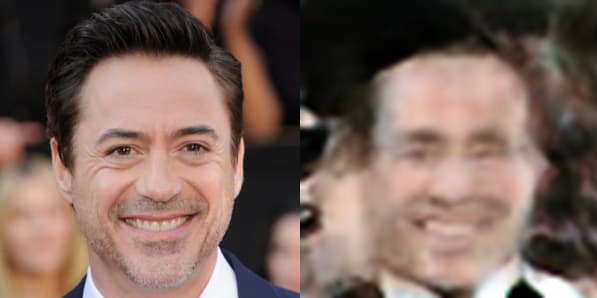
\includegraphics[width=1\linewidth]{pic/InfoBEGAN_tony_recovered_ssim}
	\caption{Iterative noise recovery (used our InfoBEGAN generator) with SSIM loss function to regenerate Tony Stark}

\end{figure}

To further improve the image quality, especially when generating 128x128 pixel images, we used the Multi-scale Structural Similarity method (Fig. \ref{fig:ms_ssim}).

\begin{figure}[!htb]
	\centering
	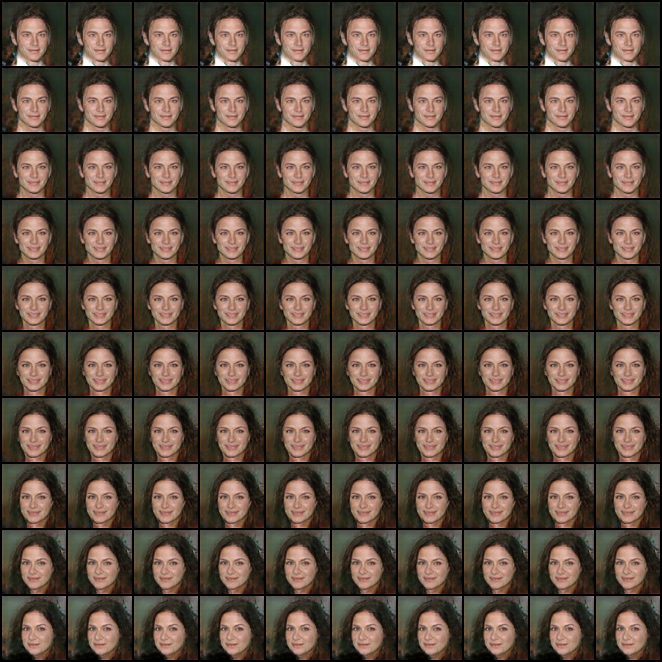
\includegraphics[width=1\linewidth]{pic/InfoBegan_varied_result}
	\caption{Controlled image generation from noise with InfoBEGAN and noise predictor}
	
\end{figure}

We also used these functions to iteratively approximate the to-be-predicted noise vector and the limit of recovery.



\subsection{Improving image quality of Info-BEGAN with VGG-based image embedding}

After we experimented with multiple quality improving methods we found a new and promising one: instead of comparing the original and recovered images pixel-by-pixel we can embed them into a feature space and compute their distance in that space.
\\

\begin{figure}[!htb]
	\centering
	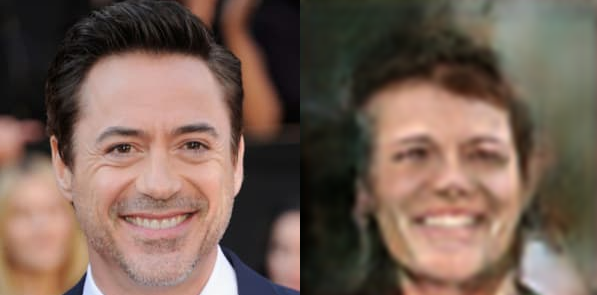
\includegraphics[width=1\linewidth]{pic/InfoBEGAN_tony_recovered_VGG16}
	\caption{Iterative noise recovery (used our InfoBEGAN generator) with VGG-16 feature layers to regenerate Tony Stark}

\end{figure}

To implement this kind of image comparison multiple source \cite{abdal2019image2stylegan} uses the first few layers of the VGG-16 image classification network because these convolutional layers can detect low-to-mid level image features and can create a meaningful latent space.



We modified our image evaluation method to first make this embedding then compute L2-distance between the resulting vectors. We used the first 23 layers of the feature extractor part, then flattened the 14x14x512 sized output.

This idea of using image embedding to determine a meaningful distance metric for images needs further development because we see great potential in it but had no time to complete the integration of it.


\section{Results}
The results were not as satisfying as we wanted. It seems the InfoGAN architecture is focused only on the maximization of the mutual information and not to produce visually pleasing images. We also noticed, that for a good prediction the Noise Predictor needs to have a Generator that can produce images with good quality. Also, the resolution is important, because we tried both 64x64 and 128x128 images, and the bigger resolution led to better quality of reconstruction. At this area we had to handle a trade-off because the better-quality demand much more compute performance or much more training time. We trained our model with a Nvidia TitanX P with 12GB GPU memory. We completed more than 30 training and several of them was over 30 hours.



On our results obviously visible the bad generation and quality caused fault. Some part of the result pictures contains the information what we want, but overall the generated images are not usable for data augmentation yet.

\section{Future plans}
To improve the generation quality, we will try to further develop the Info-BEGAN architecture and continue experimenting with image embedding. Further hyperparameter optimization is also considered due to lack of time to optimize the latest architecture. We hope we can develop a highly controllable generator on the foundation laid by these extensive experiments conducted during this semester.


\begin{thebibliography}{1}

\bibitem{goodfellow2014generative}
I.~J. Goodfellow, J.~Pouget-Abadie, M.~Mirza, B.~Xu, D.~Warde-Farley, S.~Ozair,
A.~Courville, and Y.~Bengio, ``Generative adversarial networks,'' 2014.

\bibitem{radford2015unsupervised}
A.~Radford, L.~Metz, and S.~Chintala, ``Unsupervised representation learning
with deep convolutional generative adversarial networks,'' 2015.

\bibitem{chen2016infogan}
X.~Chen, Y.~Duan, R.~Houthooft, J.~Schulman, I.~Sutskever, and P.~Abbeel,
``Infogan: Interpretable representation learning by information maximizing
generative adversarial nets,'' 2016.

\bibitem{10.1007/978-3-319-78452-6_5}
D.~Kim, H.~Jung, J.~Lee, and J.~Kim, ``Improved infogan: Generating high
quality images with learning disentangled representation,'' in \emph{Robot
	Intelligence Technology and Applications 5}, J.-H. Kim, H.~Myung, J.~Kim,
W.~Xu, E.~T. Matson, J.-W. Jung, and H.-L. Choi, Eds.\hskip 1em plus 0.5em
minus 0.4em\relax Cham: Springer International Publishing, 2019, pp. 43--48.

\bibitem{mirza2014conditional}
M.~Mirza and S.~Osindero, ``Conditional generative adversarial nets,'' 2014.

\bibitem{liu2019stgan}
M.~Liu, Y.~Ding, M.~Xia, X.~Liu, E.~Ding, W.~Zuo, and S.~Wen, ``St-gan: A
unified selective transfer network for arbitrary image attribute editing,''
2019.

\bibitem{berthelot2017began}
D.~Berthelot, T.~Schumm, and L.~Metz, ``Began: Boundary equilibrium generative
adversarial networks,'' 2017.

\bibitem{1292216}
Z.~{Wang}, E.~P. {Simoncelli}, and A.~C. {Bovik}, ``Multiscale structural
similarity for image quality assessment,'' in \emph{The Thirty-Seventh
	Asilomar Conference on Signals, Systems Computers, 2003}, vol.~2, Nov 2003,
pp. 1398--1402 Vol.2.

\bibitem{zhao2015loss}
H.~Zhao, O.~Gallo, I.~Frosio, and J.~Kautz, ``Loss functions for neural
networks for image processing,'' 2015.

\bibitem{abdal2019image2stylegan}
R.~Abdal, Y.~Qin, and P.~Wonka, ``Image2stylegan: How to embed images into the
stylegan latent space?'' 2019.

\end{thebibliography}

\end{document}
%%%%%%%%%%%%%%%%%%%%%% end of EgPublSamp.tex %%%%%%%%%%%%%%%%%%%%%%
